\documentclass[twoside,openright]{uva-bachelor-thesis}

%\usepackage[dutch]{babel}  % uncomment if you write in dutch
\usepackage{graphicx}
\usepackage{url}
\usepackage{mathtools}
\usepackage{amsmath}


% Title Page
\title{The Giving Game}
\author{Julian Ruger}
\supervisors{Peter Weijland (UvA)}
\signedby{}


\begin{document}
\maketitle

\begin{abstract}
This is the abstract. 
\end{abstract}

\tableofcontents

\chapter{Introduction}
In today’s world money is the primary medium of exchange. Money is used to express the value of a transaction and is the major source of wealth. It’s almost impossible to imagine an economy where no currency is used, even though it’s more common than one may think. In this world goods are given away without a currency to express its value. People often do not perceive giving as an economic transaction. On the contrary, giving is capable of establishing a whole independent economy. 

With today’s technology giving is becoming an even more common occurrence. The internet is an important environment for communities where money is not used as a medium of exchange. File sharing and the availability of open-source software is a great example of such a giving economy. On a more a more smaller scale giving is commonly used within communities of family and friends. Within these kind of communities giving away a good is not perceived as a direct loss, but instead it is expected that something will be given in return in the future. The value of transactions within such communities are determined by the relationship between the two participating parties of a transaction. People who have a better relationship with each other than with someone else value each other’s transactions more. 

The purpose of this thesis is to research the behaviour of people within an economy of giving under certain conditions. For example In real life people often seem to prefer to give to friends and family rather than to strangers. Thus they value a transaction with them more than with others. Under certain conditions people will assign a preference to a person or persons to who they will give to. 

\section{Contribution}
This thesis will research the behaviour of people within a giving economy from a more game theory oriented perspective. A giving game designed by P.W. Weijland will be used to simulate an economy of giving. The goal of this thesis is to create a simulation program that can simulate a giving game of N agents and M goods. 
\\
\\
Chapter 2 will show the theoretical background of giving and the giving game. At the end of chapter 2 the research questions will be explained. Chapter 3 will describe the giving game used for this thesis and will show the simulation model that will be used to simulate this giving game. Chapter 4 will show the implementation of the giving game. The technical side of the simulation will be explained. Chapter 5 will describe the scenarios that will be used for the simulation. Chapter 6 will show the results of the scenarios from chapter 5. Chapter 7 discusses these results and answers the research questions. Lastly chapter 8 will suggest further research that can be accomplished with this thesis and the created simulation model.




\chapter{Theoretical background}
Giving is a more complex process than one may think. Firstly giving can be interpreted in multiple ways.
\begin{itemize}
  \item Giving can be giving something without getting something in return
  \item Giving can be giving something and getting something in return in the future.
  \item Giving can be a trade where something is giving and something is received.
\end{itemize}
When giving the value of the good is perceived by everyone differently. This means that when two goods are traded both goods do not necessarily need to be of the same value. To express the value of a transaction an economy of giving uses social credit. The social credit is an indication of the relationship between two people. Every individual keeps track of their own social credit balance with every other person and bases their perception of the value of a transaction on this credit balance.

Based on this social credit people can have multiple reasons to give away something, but giving is almost always with the intention to get something in return. As shown in the article ‘Giving with Impure Altruism: Applications to Charity and Ricardian Equivalence’ even giving to charity is often not completely selfless. When giving out of kindness or the help someone else most people still get a good feeling when giving. The article calls this feeling the ‘warm glow’. This shows that giving can still be with the intention to get something in return even if it seems to be out of kindness. This also shows that what is given in return does not have to be of the same value and that some people value giving to charity more than others, because of their perception of what they get in return.

In real life people often seem to prefer to give to friends and family rather than to strangers. Thus they value a transaction with them more than with others. Under certain conditions people will assign a preference to a person or persons to who they will give to. When the transactions only take place in a certain group a community effect emerges.

The behaviour of people in an economy of giving can be a lot more complex than in an economy where money is used as a medium of exchange. With money it is easy to express a value of a transaction and almost everyone perceives this value the same. With giving this value is based upon multiple factors and can be different for every person.



\section{The economic model}
In the article ‘Money Network in Kiyotaki-Wright Model’ an environment with three agents and three goods is simulated. Each agent produces one good and consumes another. This article shows the behaviour of the agents when they want to trade their good for the good they need to consume. This simulation used an economy environment without money, but only focused on scenarios where agents only give away their good if they get a good in return which they can use. 
\\
\\
P.W. Weijland has created a similar model called ‘The Giving Game’, but instead focuses on more aspects of giving. A giving game is a game to simulate giving in real life. A giving game can be very versatile and a lot of variants are possible to simulate different real life economic environments. In this section the basic rules of a giving game are explained and the giving game used for this thesis is explained.
The following rules show the basics of a giving game:
\begin{itemize}
  \item In an environment of N agents an agent is randomly chosen to start with a good.
  \item Once an agent has the good the agent is meant to give it to someone else.
  \item Each time an agent receives the good the agent receives a credit point.
\end{itemize}

This thesis uses a variant of this giving game to simulate the behaviour of giving in real life under certain conditions.

\section{Yield curve}
Every agent values the transaction of a certain good differently for each agent. This value of the transaction is called the yield. The yield is calculated using the account balance (social credit), the like factor and the nominal value of a good. The like factor is an indication of the relationship between two agents. The higher the value the better the relationship. The nominal value is perceived differently by every agent.
The following function is used to calculate the yield:
\\
\\
\textit{Y = a*x + b} \\
\textit{-1 $\le$ a $\le$ 0} \\
\textit{Y, b $\ge$ 0} \\
Here is \textit{a} the like factor, \textit{X} is the account balance and \textit{b} is the nominal value of a good. With this function we can create a yield curve as follows.
\\
\textbf{Image of yield curve here}
\\
Every agent keeps track of their account balance in relation with the other agents. This means that agent P can have a different balance with Q than with R. The balance is an indication of how much an agent has given and received. From the yield curve it is clear that when the account balance of P with Q gets higher the yield gets lower. This can be interpreted as the more P gives to Q the higher the balance of P with Q thus the more P is ‘in the black’ with Q and the more Q is ‘in the red’ with P. This means that Q is in debt with P. The balance after a transaction is calculated by adding the yield of that transaction to the current balance. When the yield gets lower the balance increases less, so for the next transaction the yield will also decrease less. The yield will never reach zero.

The yield will be important to determine who will receive a good next. If P would for example want to maximize its profit P would only want to give away a good to someone with who P has a high yield. Agents who are in debt with P and are not likely to pay of this debt would be worthless to P in this case. It would be a bad investment if P would give to these agents.
\\
\\
The yield curve can either be used to predict the course of the transactions or to see an equilibrium arise. When an equilibrium arises the yield of a good between two agents switches between two values.  Both agents perceive the transactions with each other as the most valuable and will keep giving to each other. These agents have established a community with each other and this community will hold as long as the current condition do not change. 

\textbf{Image of yield curve with equilibrium here}

\section{Research questions}
\textbf{WORK IN PROGRES!}
As explained earlier, in real life people seem under certain conditions to prefer to give to 'friends' than to strangers. This has led to the following research question:
\\
\\
\textit{Will the transactions eventually take place within a limited subgroup of the entire population?}
\\
\\
If no community effect emerges the transactions can still fall into a repeating sequence of transactions. This has led to the second research question:
\\
\\
\textit{Will we see a repeating sequence of transactions or will the transaction sequence look random?}


\chapter{Design}
For this thesis the giving environment consists of a fixed amount of agent and a fixed amount of goods. For every simulation the number of agents and number of goods can be changed, but during the simulation no agents or goods are added or removed.  Every agents keeps track of their own account balance and transaction values in relation to every other agent. The agents don’t know anything about each other, they operate completely independent.

There are two types of goods, ‘sustainable’ and ‘perishable’ goods. ‘Sustainable’ goods are goods that will exist for eternity. ‘Perishable’ goods are goods that perish after a certain amount of transactions. Every ‘perishable’ good has a producer. The producer is also an agent in the environment so the producer also participates in transactions of other goods. The producer reproduces its ‘perishable’ good after a certain amount of time the good has perished. The value of a good is valued differently by each agent, but this value does not change during the simulation. For the experiments in this thesis the agents are not able to hold on to a good for a certain amount of time. This is a variant which can be used in further research. Holding on to a good will be explained further in the last chapter. At the start of the giving game the goods can either be divided randomly over the agents or are divided by hand. The agents who start with the perishable goods are assigned to be the producers.

The transactions can be executed in two different ways. The transactions can be executed one by one which is a more game theory based approach. A more realistic approach is that the transactions are executed simultaneously, this way agents don’t have to wait for each other before they can give away their good. Both types are used in the experiments.

The emergence of a community effect is determined by the amount of transactions each agent is part of. When more than one good is used in the environment there can emerge multiple communities. That is why every good is looked at independently. Every agent keeps track of their own transactions and how much they have traded each good. If for example two agent hold 100 percent of the transactions of good A and two other agents hold 100% of the transactions of good B then two separate communities of size two have emerged. There can be concluded that the community effect exists for this scenario. If this time two agents hold 50 percent of the transactions of good A and good B and two other agents also hold 50 percent of the transactions of good A and good B than this means that one community has emerged with a size of four. There can also be concluded that a community effect exist in this scenario.  A community effect can exists as long as the size of the subgroup is smaller than the total amount of agents in the environment and 100 percent of the transactions of one or more goods takes place inside this subgroup. This means that even if an agents holds a smaller percentage of the transactions this agent can still be part of the community as long as the previous stated rules apply.

The stabilization of the transactions in the environment can be determined by predicting future transactions. If multiple transactions in a row can be predicted or if a pattern is clearly visible than there can be concluded that the transactions have stabilized. The emergence of a community does not mean that the transactions are executed in a repeating sequence. Even in a community the transactions can be executed randomly.


\section{Paramaters}
The following parameters will be used in the environment of the giving game for the experiments.

\begin{description}
  \item[N:] The number of agents used in the simulation
  \item[M:] The number of goods used in the simulation
  \item[Perish period:] The perish period is the amount of transactions it takes before a good perishes. For sustainable goods the perish period is 0, because sustainable goods exist forever. For perishable goods the perish period is greater than 0. For example, when a good has a perish period of 3 then this good can be given away 3 times before it perishes. The perish period is a natural number greater than or equal to 0.
  \item[Production delay:] The production delay is the time between the perish of a good and its reproduction. The time until the production is decreased by one after every iteration over all agents who are currently holding a good. The production delay is a natural number greater than or equal to 0.
  \item[Nominal value:] The nominal value is an indication of how much a good is worth. The nominal value does not change during the giving game. Every agent perceives the nominal value of a good differently. Agent P could value good G more than agent Q for example. The nominal value is a natural number greater than or equal to 0.
  \item[Like factor:] The like factor is a real number between -1 and 0 which defines how much agent P likes agent Q. The higer the number the more P likes Q the more likely it is that P will give to Q if the like factor is used in the selection rule. The like factor does not change during the giving game. 
  \item[Selection rule:] The selection rule is an algorithm that decides/calculates the next agent who should receive a good.

\end{description}

\section{Selection rules}
For every transaction the selection rule decides which agent will receive a good. This decision is based on different parameters of the giving game. These selection rules simulate  multiple real world scenarios for example: choosing the agent based on maximizing the profit (goodwill rule).

\subsection{Random rule}
The random rule is the most basic rule for the giving game. The agent who should receive the good during the transaction is chosen randomly. The random rule simulates an environment where the agents do not care about the value of the goods and do not care about who will receive the goods. The \textit{like factor} is therefore 0 for every agent pair. This leads to the following yield curve. This rule is mostly used to see if the giving game enviroment behaves as it should.

\subsection{Balance rule}
A more advanced selection rule is the balance rule. The agent who should receive the good during the transaction is chosen based on the balance between the giving agent P and the receiving agent Q. Agent P chooses agent Q if P has the highest balance with Q. If P has the same highest balance with multiple agents then the receiving agent is chosen randomly between these agents. The balance rule simulates an environment where each agent only gives to the agent from who they have received the most. Agent P tries to maximize the number of goods he receives. The balance in this case can be calculated as follows: 
\\
\\
\textit{Balance of P with Q = Number of goods received from Q – Number of goods given to Q} \\
The following rule applies:\\
\textit{Balance of P with Q = - (balance of Q with P)}\\
This calculations of the balance is different from the calculation of the balance for the yield curve.\\

\subsection{Goodwill rule}
The goodwill rule is a more realistic rule. The agent is chosen based on the value of the transaction (the yield) between P and Q perceived by P. Only the agent where the yield is the highest is chosen as the receiving agent. If multiple agent pairs have the same yield the receiving agent is chosen randomly between these agents. Every time P gives good G to Q the value of the transaction of good G (the yield) decreases. As long as Q does not give good G to P, P loses interest in giving good G to Q. Eventually P will stop giving to Q, because P does not expect that Q will ever pay of his debt. The like factor as explained earlier defines how many transactions P can tolerate without getting anything in return from Q. For the goodwill rule the like factor can be set by the user or can be created randomly. The goodwill rule simulates an environment where every agent tries to maximize its profit. Agents who are in debt will less likely receive a good, they are not worth investing in.
This leads to yield curves that look like this: \\
\textbf{2 Yield curves of y = a * x + b where a $\le$ 0 and b $>$ 0, one yield curve is mirrored in the y-axis}\\
The steeper the slope for YP the less tolerant P is. In this case the balance is calculated as explained before.

\section{Simulation model}
For the previously explained giving game a simulator will be created that can simulate different scenarios using the parameters and selection rules. The following flow chart shows the actions that are executed to simulate the giving game.

\textbf{Image of the flow chart here, similar to the flow chart from the design document}

The technical side of the simulator will be explained in the next chapter. 


\chapter{Implementation}
\textbf{Work in progres!}
\section{The simulation model}
The simulator had to be able to execute multiple tasks. The simulator must be able to accept user input to simulate multiple scenarios. The simulator should provide a visualization module to visualize the data and to also visualize the course of the transactions. The following shows the simulation proces:

In the following sections the design choices are explained to achieve the ...
\subsection{Input}
The user is able to input the following parameters:

\begin{description}
  \item[N:] 
  \item[M:] 
  \item[Perish period:] 
  \item[Production delay:]
 \item[Selection rule:] 
  \item[Nominal value:] The user is able to choose if every agent perceives the value of a good differently or not. If the user wants to have a different value of the good for every agent the user can add a xslx file with the nominal values as follows:
  \item[Like factor:] The user is able to choose between setting like factors by hand or to randomly create the like factors. If the user wants to add predefined likefactors the user can add a xslx file with the like factors as follows:
 \item[Balance:] The use is able to set the balance at the start of the simulation at 0 or to add different balances for every agent.
\end{description}
During the simulation the user should be able to adjust the following variables:

\begin{description}
  \item[Subgroup size:] 
  \item[Reset community percentage:] 

\end{description}
\subsection{Output}
The output data is visualized so that the user is able to analyse and get results without doing any calculations. The simulator is able to do most of the work.

The simulator is able to give the following output:
\begin{itemize}
  \item Show the amount of goods given and received for each agent in a bar plot.
  \item Show the yield curve between every agent pair.
  \item Show the amount of transactions
  \item Show the visualization of the course of the transactions with a color indication for any emerging subgroups.
  \item Show percentages of how many times a certain good has been traded by an agent.
  \item Show every transaction, producting and delay in production.
  \item Show the community percentage (How many transactions take place in a subgroup with the current set size.)
\end{itemize}

All the data can be saved and used in the future for another simulation.

\section{GUI}

\section{Back-end}

\subsubsection{Python}

\section{Front-end}
The front end provides the interface between the user and the back end. With this interface the user is able to put data into the simulation to simulate different scenarios. The interface is able to visualize the responses of the back end to analyse the resulting data during the simulation.

For the explanation of the use of the interface the use should consult the user manual.


\chapter{Scenarios}
For every selection rule multiple scenarios have been created that will represent a real life situation as much as possible or will make use of as much different variables.  This chapter will explain the scenarios used in the experiments. For every experiment the results are shown to show any additions to other experiments that derived from these results.
For every experiment 99 agents will be used. 99 agents is large enough to have as much variety in the parameters as possible but is still be able to clearly see any changes in the visualisation. 99 agents is also a reasonable size that can be used in further research for example with real life behavioural experiments. Linkje naar artikel Another reason for 99 agents is that for the scenarios for goodwill rule the population will be split into 3 groups.

\section{Basic Scenarios}
For every selection rule the behaviour is tested in the most basic environment. These scenarios will be used to see if the simulation behaves as it should.
\subsubsection{Basic scenario 1, sustainable (BS\_S):}
Parameters:
\begin{itemize}
\item	99 agents
\item	1 sustainable good with a nominal value of 1, perish time of 0, perish delay of 0
\end{itemize}
\subsubsection{Basic scenario 2, perishable (BS\_P):}
Parameters:
\begin{itemize}
\item	99 agents
\item	1 perishable good with a nominal value of 1, perish time of 1, perish delay of 1
\end{itemize}
In case of the goodwill rule where the like factor is used for the selection of an agent the like factor is set to -1 for every agent. In the most basic environment every agent is equal and has no specific relations with other agents.

\section{Random rule}
Because agents are chosen randomly the results will most likely not be very meaningful. The following scenarios are therefore used to see if the agents behave as predicted with the random rule.  Any irregularities in the behaviour will be analysed and can be used in decisions for further experiments.
\subsubsection{Scenario 1, sustainable (RR\_S):}
Parameters:
\begin{itemize}
\item	100 agents
\item	3 sustainable good with a nominal values of [1,2,3], perish time of 0, perish delay of 0
\end{itemize}
\subsubsection{Scenario 2, perishable (RR\_P):}
Parameters:
\begin{itemize}
\item	100 agents
\item	3 perishable goods with a nominal values of [1,2,3], perish time of [1,2,3], perish delay of [1,2,3]
\end{itemize}
The choices for the values of the goods are based on the idea of having a small, medium and large product even though the nominal value does not affect the selection of an agent. The amount of goods is not a fixed amount, during the experiments the amount of goods will differ to see if this affects the results.

\subsubsection{Hypothesis}
It is expected that no community effect will arise, neither will the simulation stabilize even though a machine is pseudorandom. The transactions will eventually be equally distributed over all the agents. For perishable goods this distribution will be in favour of the producers, because they will be able to give away their good more than others.

\section{Balance rule}
The scenarios for the balance rule will be used to see how people will behave when they care about how many goods they give and receive but do not have any relationship with other agents.
\subsubsection{Scenario 1, sustainable (BR\_S):}
Parameters:
\begin{itemize}
\item	100 agents
\item	3 sustainable good with a nominal values of [1,2,3], perish time of 0, perish delay of 0
\end{itemize}
\subsubsection{Scenario 2, perishable (BR\_P):}
Parameters:
\begin{itemize}
\item	100 agents
\item	3 perishable goods with a nominal values of [1,2,3], perish time of [1,2,3], perish delay of [1,2,3]
\end{itemize}
The choices for these values of the goods are based on the idea of having a small, medium and large product. The amount of goods is not a fixed amount, during the experiments the amount of goods will differ to see if this affects the results.

\subsubsection{Hypothesis}
The expectations are that a community effect will arise with a subgroup consisting of a few agents. The size of this subgroup is based on the type of goods and the amount of goods. All sustainable goods will eventually be traded only between two agents, because these two agents have the highest balance with each other. Every perishable good has a producer, these producers will also be part of a subgroup. If these producers only give each other their goods then the subgroup size will be as large as the amount of producers. If the producers each give to another agent then multiple subgroups will arise with a size of two. It is expected that the maximum size of a subgroup will be the number of producers plus one non-producer who trades with the producers.

\section{Goodwill rule}
For the goodwill rule all parameters can affect the results. The following parameters define the scenarios.
\subsubsection{Like factors}
\begin{description}
\item[L1]	1/3 of the population has a like factor of -1, 1/3 of the population has a like factor of -0.5 and 1/3 of the population has a like factor of -0.1. This means that every agent has a different relationship with every third of the population.
\item[L2]	47 agents have a like factor of -1, 47 agents has a like factor of -0.5 and 5 of the agents have a like factor of -0.1. This means that only a small group of agents is liked by all other agents.
\end{description}
\subsubsection{Balances}
\begin{description}
\item[B1]	At the start of the simulation all account balances are set to 0.
\item[B2]	At the start of the simulation all account balances are randomly set. The account balance will vary between -9 and 9.
\end{description}
\subsubsection{Nominal values}
\begin{description}
\item[N1]	The nominal values of every good are the same for every agent.
\item[N2]	Every third of the agents perceives the nominal values of all goods differently, with the values increasing. Just like the like factors, the population is divided into 3 groups, where every group perceives the value of the goods differently.
\end{description}
The combination of these parameters will form different scenarios. Every combination will be tested unless previous experiments show that one of the parameters does not affect the result. The scenarios are based on the idea of having a population where people have different relationships with each other and value goods differently. That’s why the population is split into 3 groups to have groups that are completely different from each other.The following scenarios will be used during the experiments.
The first scenarios are scenarios where the balance is zero.
\begin{description}
\item[GR\_L1B1N1], Goodwill rule using L1, B1 and N1 as input.
\item[GR\_L1B1N2], Goodwill rule using L1, B1 and N2 as input.
\item[GR\_L2B1N1], Goodwill rule using L2, B1 and N1 as input.
\item[GR\_L2B1N2], Goodwill rule using L2, B1 and N2 as input.
\end{description}
After these scenarios B2 will be used for the balances.
\begin{description}
\item[GR\_L1B2N1], Goodwill rule using L1, B2 and N1 as input.
\item[GR\_L1B2N2], Goodwill rule using L2, B2 and N2 as input.
\item[GR\_L2B2N1], Goodwill rule using L1, B2 and N1 as input.
\item[GR\_L2B2N2], Goodwill rule using L2, B2 and N2 as input.
\end{description}
 Work in progress!

\subsubsection{Hypothesis}


\chapter{Experiments}

\section{Random rule}
The scenarios mentioned in the previous chapter are used in the simulator. Changing the amount of goods did not change the results.
\subsection{Results}

\subsubsection{BS\_S}
No community effect arose and the transaction also did not stabilize. The transactions are still completly random. After 100000 transactions the distribution of the transactions was between 0.9 and 1.1 percent for each agent. More transactions will lead to more equally distributed transactions.

\subsubsection{BS\_P}
The producer participated in 50 percent of the transactions, because after each time the producer give away its product it perishes. The other agents only received the good during this scenario. The producer kept choosing the receiving agents at random. The other 50 percent of the transactions (the receiving part) is distributed oer the other 99 agents. Each agent participated in approximately 0.5 percent of the transactions. No community effect arose and the transacitons did not stabilize.
\textbf{IMAGE OF THE DISTRIBUTION OF THE TRANSACTION HERE}

\subsubsection{RR\_S}
The results are similar to the results from RR\_N1. No community arose, neither did the transactions stabilize. All the transactions of each good were distributed over all agents. Each agent participated between 0.3 and 0.35 percent of the transaction of each good.

\subsubsection{RR\_P}
The results are similar to the results from RR\_N2. No community arose, neither did the transactions stabilize. Good\_1 is the good with the lowest perish period and the lowest production time. This good was therefore participated the producer of this good in approximately 16.7-16.8 percent of the transactions of this good. The producer of Good\_2 particiated in approximately 8.4 percent of the transactions of Good\_2, which is half of 16.8 percent. This makes sense, because the perish period and production delay of Good\_2 is twice the amount of the perish period and production delay of Good\_1. The producer of Good\_3 particiated in approximately 5.7 percent of the transactions of Good\_3, which is almost a third of 16.8 percent. This makes sense, because the perish period and production delay of Good\_3 is three times the amount of the perish period and production delay of Good\_1. 
These numbers are the results after 20000 transactions. \\
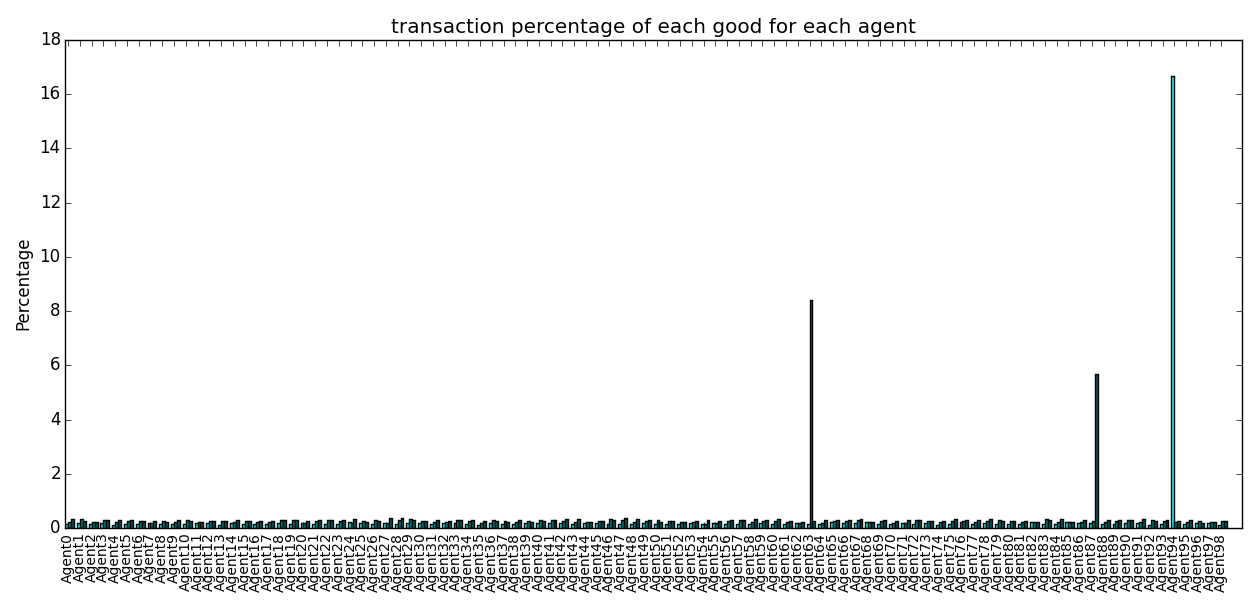
\includegraphics[scale=0.5]{experiment_images/RR_P}

\section{Balance rule}
All the scenarios mentioned in the previous chapter have been tested. Changing the amount of goods did not lead to different results.
\subsection{Results}

\subsubsection{BS\_S}
Every time an agent receives the good the receiving agent gives the good back to the giving agent during the next transaction. The moment P gives Q the good Q has the highest balance with P, because Q has received more from P then Q has given to P. This means that Q will give the good to P during the next transaction and all agents have now the same balance with P again. Now P has to choose randomly who should receive the good next. No community arises, but the simulation is partially stabilized. It is partially stabilized because P will always get the good back after P has given it away. The only thing that is still random is the choice for P to who P should give to. \\
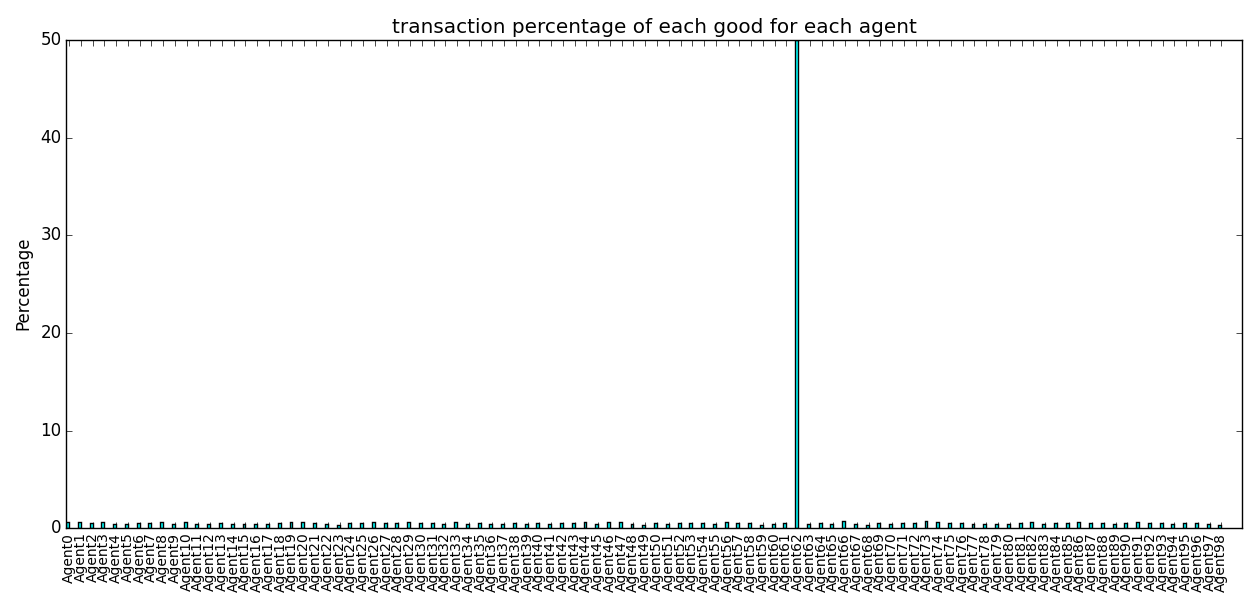
\includegraphics[scale=0.5]{experiment_images/BR_BS_S}

\subsubsection{BS\_P}
The producer participated in 50 percent of the transactions, because after each time the producer give away its product it perishes. Each other agent participated in approximately 0.5 percent of the transactions. The moment the producer gives the good to let's say agent Q the balance of the producer with Q is now lower then the balance of the producer with all other agents. This means that the next transaction the producer will not give to Q but has to choose randomly between all the other 98 agents, because the balance of the producer with the other agents is equal to each other. The same happens after the next transactions, now the producer has to choose randomly between 97 agents. This goes on untill 1 agent is left to choose from, at this point the choice is not random anymore, because only 1 agent is left. After this agent has received a good from the producer everyone is equal again and the whole process starts from the beginning. This leads to the conclusion that after every 98 transactions the next transaction can be predicted.  No community effect arisis, but the transactions are partially stabilized. \\
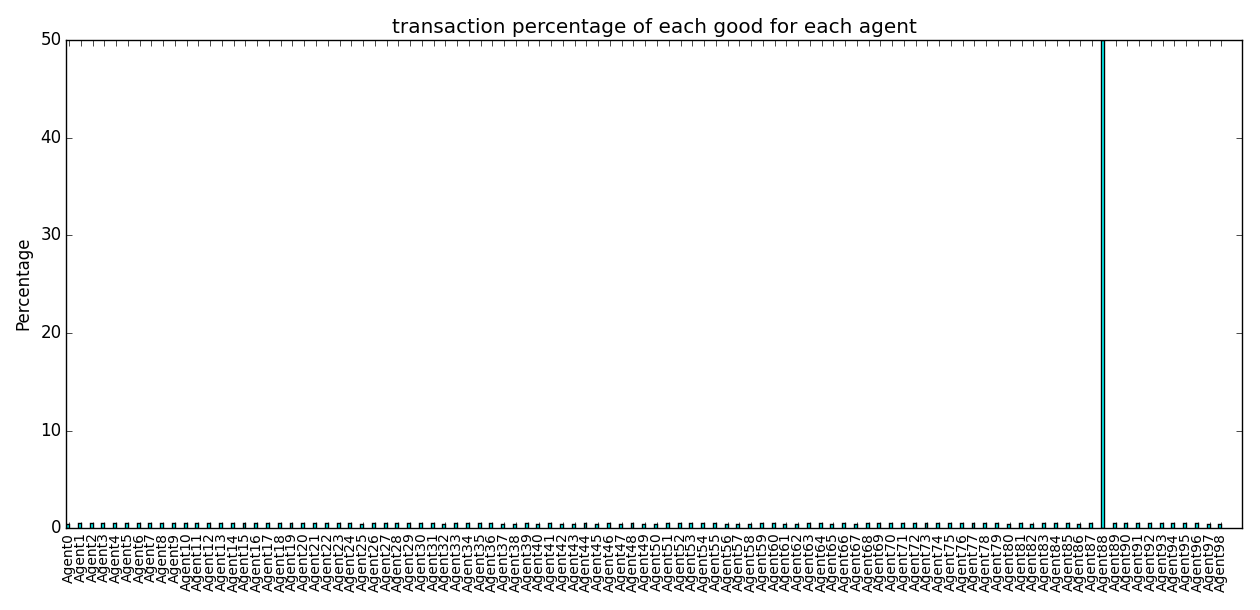
\includegraphics[scale=0.5]{experiment_images/BR_BS_P}
\subsubsection{BR\_S}
The results are quite remarkable. As expected after seeing the results from BS\_S the goods are returned to the giving agent after each transaction, but the only difference is is that the agents who start with the goods at the start of the simulation give in proportion more to each other than to the other agents. \textbf{WHY?} \\
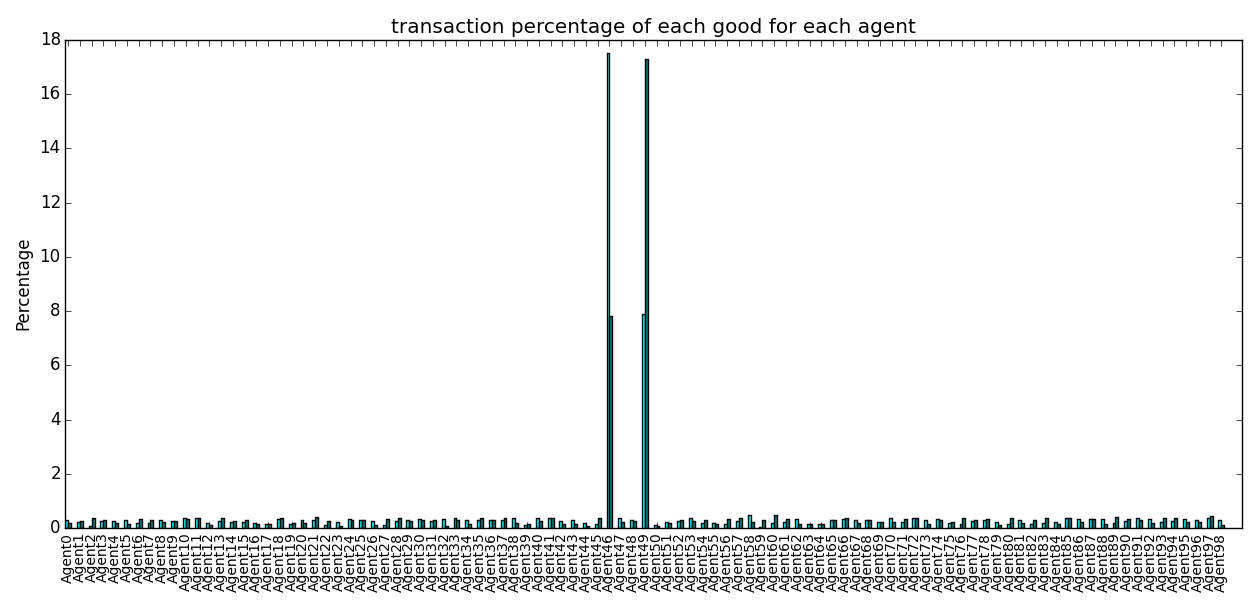
\includegraphics[scale=0.5]{experiment_images/BR_S}

\subsubsection{BR\_P}

\section{Goodwill rule}
All the scenarios mention in the previous chapter have been tested. Changing the amount of goods did change some results. These results are explained in the next sections.
\subsection{Results}

\subsubsection{BS\_S}
Immidiatly at the start of the simulation a community effect arises with a subgroup of size two. The moment agent P gives to agent Q, Q is in debt with P. This means that Q values the next transaction more with P. So Q will give to P during the next transaction. Now P values the transaction with Q more then with any other agent, so P gives back to Q. This goes on in eternity where eventully the yield of the transaction for P with Q an Q with P will switch between the same values. The following yield curve shows what happens. 

\subsubsection{BS\_P}
The value of the transactions will approach zero, but it will never reach zero, because of the way the yield is calculated. No community effect arisis, but the transactions are partially stabilized.

\subsubsection{GR\_L1B1N1}
Because all the balances are zero at the start and the nominal values are the same for everyone the yield of the first transaction is the same for everyone. The agent who first start with the good randomly gives the good to another agent. From this point on the subgroup has emerged and the good will only be traded between these agents. Good\_0 is from the beginning only traded within a subgroup of size 2.  When P gives to Q, Q is in debt with P and values giving to P more than giving to anyone else, the yield is the highest between Q and P. Q gives back to P and now the yield for P has become greater than the nominal value so P values the transaction with Q the most. An equilibrium emerged. Changing the amount of goods did not change the results. Each good is only traded between 2 agents.
\subsubsection{GR\_L1B1N2}
In the beginning some goods are traded between different agents. This happens because after some transactions the yield falls below the nominal value of an agent. If this happens the agent who is in possession of the good prefers to give to someone else. This happens between agents where their nominal value is either a multiple of the other. \textbf{More calculations here!!!} 
\subsubsection{GR\_L2B1N1}
The results are the same as the results from GR\_L1B1N1.
\subsubsection{GR\_L2B1N2}
The results are similar to the results from GR\_L1B1N2. The biggest difference is that it takes longer before all goods are traded within a subgroup. The cause of this is that the nominal values differ alot more.

These results have shown that when the nominal values are the same that a subgroup immediatly arises after the first transaction. For these scenarios the results are affected more by the nominal values than the like factors. 

\subsubsection{GR\_L1B2N1}
The first thing that the experiments with sustainable goods show is that in the beginning the transactions are mostly divided over the agents with a likefactor of -1 and -0.5. After the first 1000 transactions the transaction percentage is as follows. \\
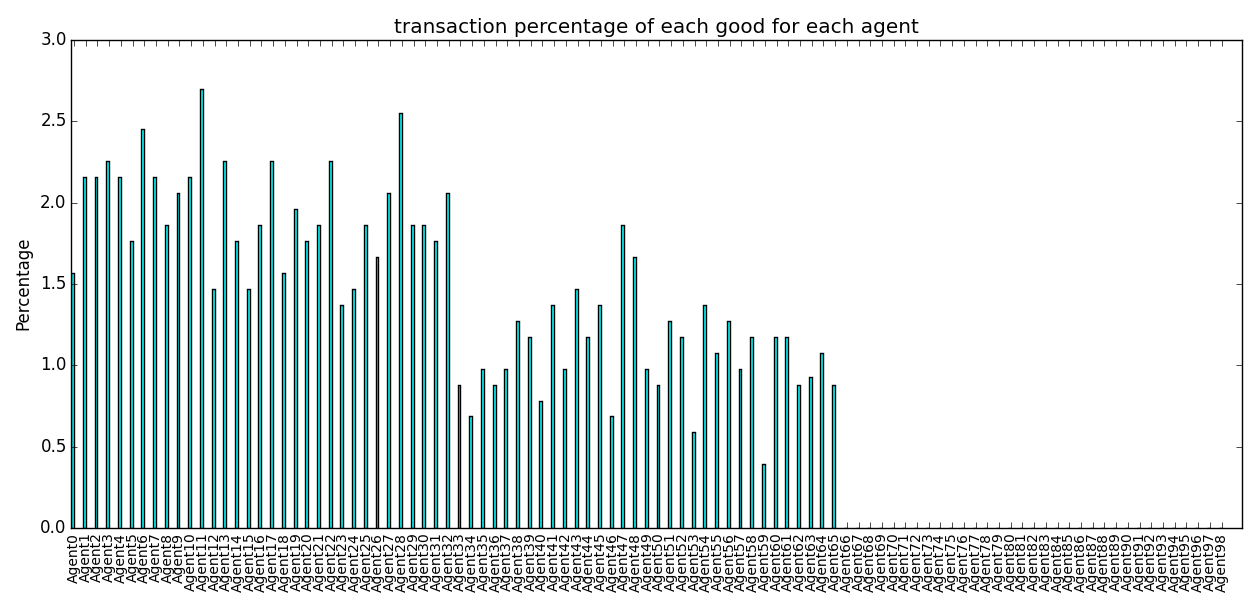
\includegraphics[scale=0.5]{GR_L1B2N1/1000transactions}
 Every experiment with just one good led to a subgroup of agents with likefactor -0.5. With just one good the good was  only traded between 2 agents after 4000-5000 transactions. When more goods are used the results start to vary alot more. One of the results which differs from the others showed a distribution of the 2 goods used as follows. \\
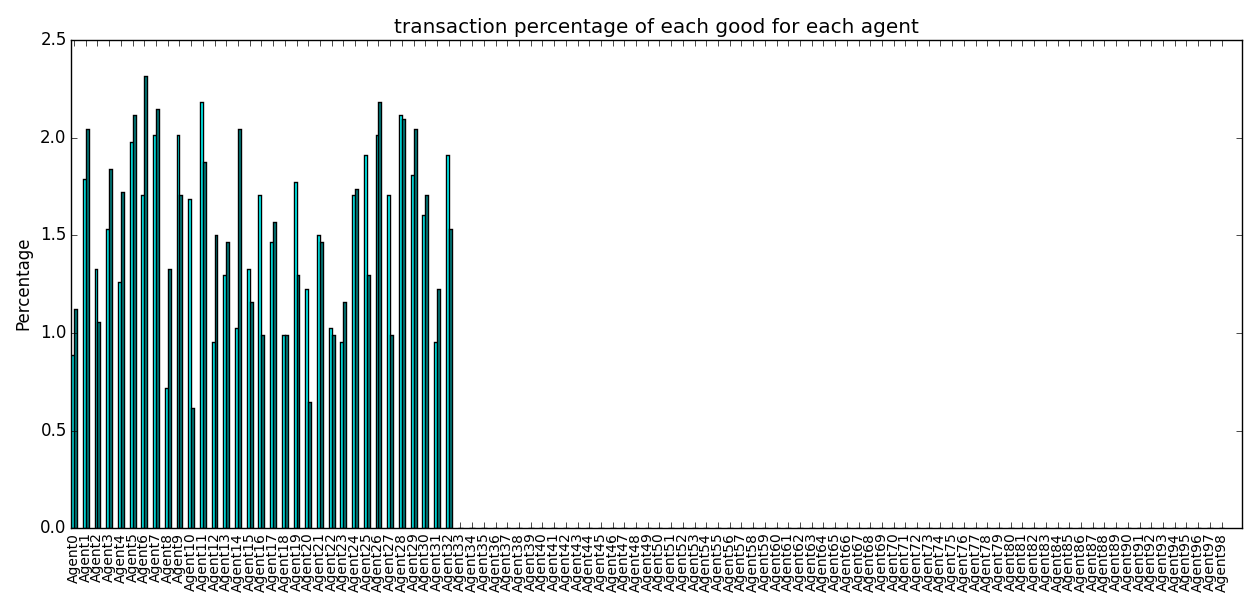
\includegraphics[scale=0.5]{GR_L1B2N1/30000transaction2}
This was after 30000 transactions. In this case a community does arise with only agents who have a like factor of -1. Even though a like factor of -1 would mean a 'bad' relationship the slope of -1 for the yield curve is the highest which means a bigger change in the yield after every transaction. Receiving a good would mean a bigger debt and giving a good would mean a bigger loss.
Other results showed a more equal distribution of the transactions or a distribution in favour of agents with a likefactor of -0.5 or -0.1. Most experiments led eventaully to communities of 2 agents. The more goods were used the longer it took for a community to arise. \\
\\
For the perishable goods the results are slightly different. With one perishable good and a perish period of 1 all experiments led to a community of the producer and all the agents with a like factor of -0.1 and -0.5. Because the good perishes after it has been given away by the producer the agents who receive the good stay in debt with the producer. The producer prefers therefore the agents with a like factor of -0.1 and -0.5 over -1. \\
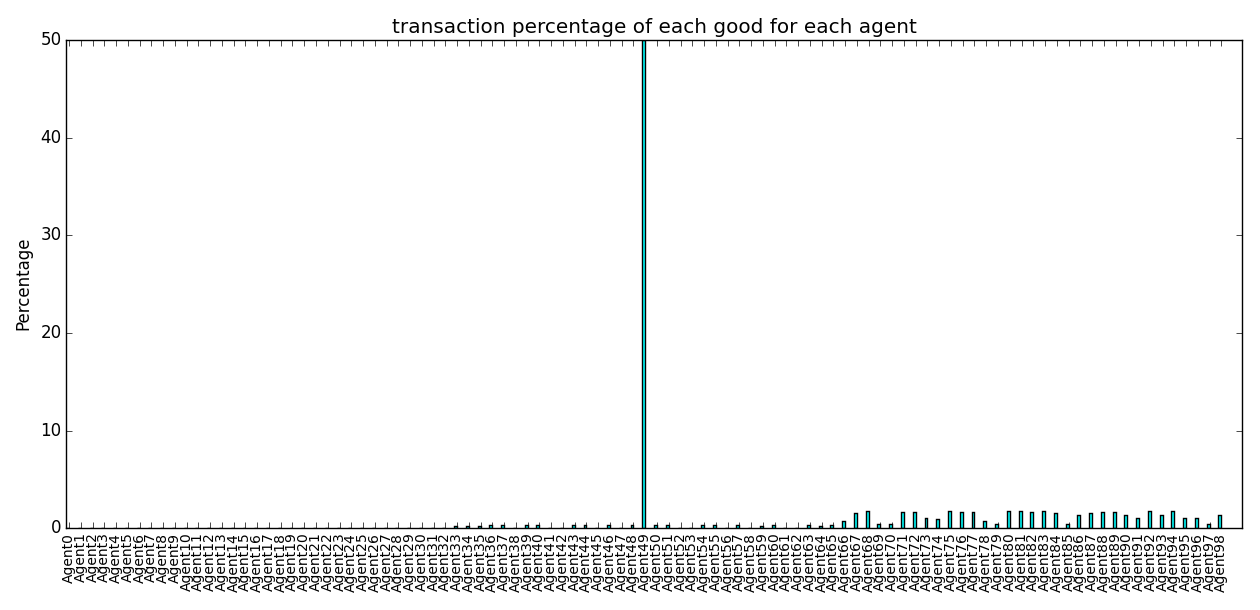
\includegraphics[scale=0.5]{GR_L1B2N1/1000transactions1perishable1-1}
When the perish period is higher than 1 the goods behave more like a sustainable good. The higher the perish period and the more perishable goods are used the longer it takes before a community arises.\\
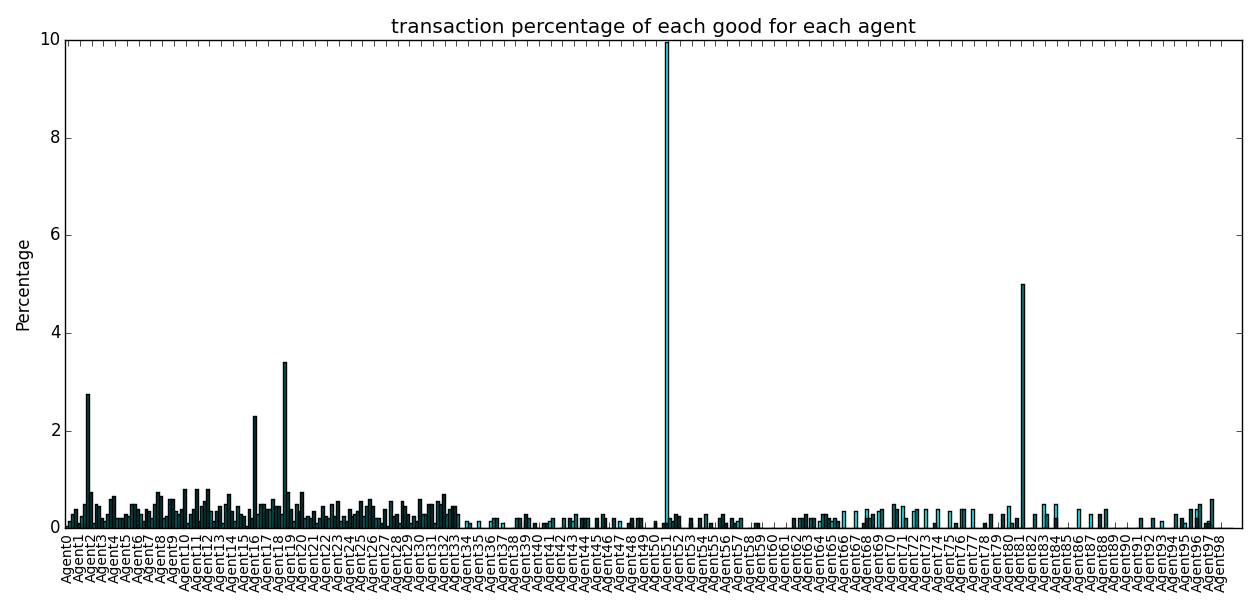
\includegraphics[scale=0.5]{GR_L1B2N1/1000transactions5perishable}
The figure above shows the distribution of the transactions of 5 perishable goods where good\_0 has a perish period of 1 and a production delay of 1, good\_1 has a perish period of 2 and a production delay of 2 etc. These results are after 1000 transactions and show that when the perish period gets higher (the darker green colored bars) the behaviour is more like a sustainable good explained above.

\subsubsection{GR\_L1B2N2}
With these experiments the nominal values are perceived differently by some agents.For the sustainable goods the results show that a community arises more quickly in comparison with GR\_L1B2N1 where the nominal values are the same for every agent. Where it took GR\_L1B2N1 with one good 4000-5000 transactions before a community arose these experiments only took 2000 transactions for one good. The distribution of the transactions is the same as with GR\_L1B2N1. 

For the perishable goods the results are the same as GR\_L1B2N1. The nominal values do not affect the behaviour.
\subsubsection{GR\_L2B2N1}
\subsubsection{GR\_L2B2N2}

The results of these scenarios have shown that for these scenarios the nominal values affect the results less, but the like factors start to play a more important role.

\chapter{Conclusions and Discussions}

\chapter{Further research}
A possible variant on the giving game used in this thesis is that agents are able to hold on to a good. This is leads to a similar simulation as used in the article 'Money Network in Kiyotaki-Wright Model'. Holding on to a good is a more realistic approach, but comes with a few extra parameters. Realistically holding on to a good means that the good needs to be stored somewhere. In the real world this would mean that storage costs have to be paid and certain goods (perishable goods) would not be able to be stored forever. The time an agent holds on to a good is also a parameter that can influence the choice for the transaction.

\chapter{Appendix A}

\section{Simulator manual}

\section{Code Documentation}



\end{document}